\documentclass[twocolumn]{jsarticle}
\usepackage[dvipdfmx]{graphicx}
\begin{document}

\title{UPPAALを用いた自動運転車の\\群制御アルゴリズムのモデル化と検証}
\author{佐原優衣}
\maketitle

\section*{背景目的}
近年自動運転の技術は発達しているため,将来的には自動運転車が実用化されると考える。多数の自動運転車が実用化された都市空間を考える。個々の車が他車を考慮しない目的地までの経路決定を行うと問題が発生する可能性がある。従って自動運転車の群制御アルゴリズムが必要となる。
先端エネルギー技術を駆使してエコシティを目指すアラブ首長国連邦の都市計画と,その計画によって建設されているマスダールシティがある。自動運転車のみが走行するマスダールシティのような現在の自動車と完全に住み分けされた都市空間を想定する。限られた空間内で多数の自動運転車が実用化された際にその群制御アルゴリズムが性質を満たしているのかを検証する。

本研究は自動運転車の群制御アルゴリズムを形式的に記述し,その性質を形式的に検証することを目的とする。
\section*{方法}
群制御アルゴリズムをオートマトンで記述し,モデル検査用いて,性質を検証する。本研究では時間オートマトンによる時間制約性質を検証できるUPPAALを使用する。
\begin{figure}
	\centering
	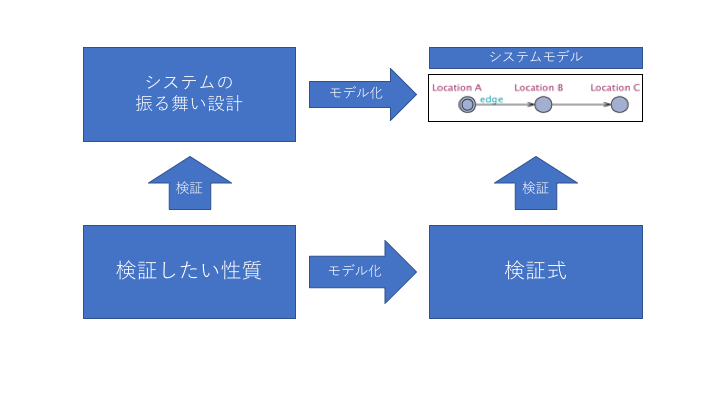
\includegraphics[width=80mm]{kensho.png}
	\caption{モデル検査とは}
\end{figure}
\section*{UPPAALによるモデル化と検証}
今回は交差点をモデル化し,衝突が起きないことと,同時通過できない方向に関して通過していないことを検証する。図2の赤い矢印が車の動線で,中央のクロスポイントを使用する際衝突を回避するためにはクロスポイントは同時に1台までしか利用できない。この性質を利用し,図3に置いてその他の衝突が防げるかどうか検証した。
\begin{figure}
	\centering
	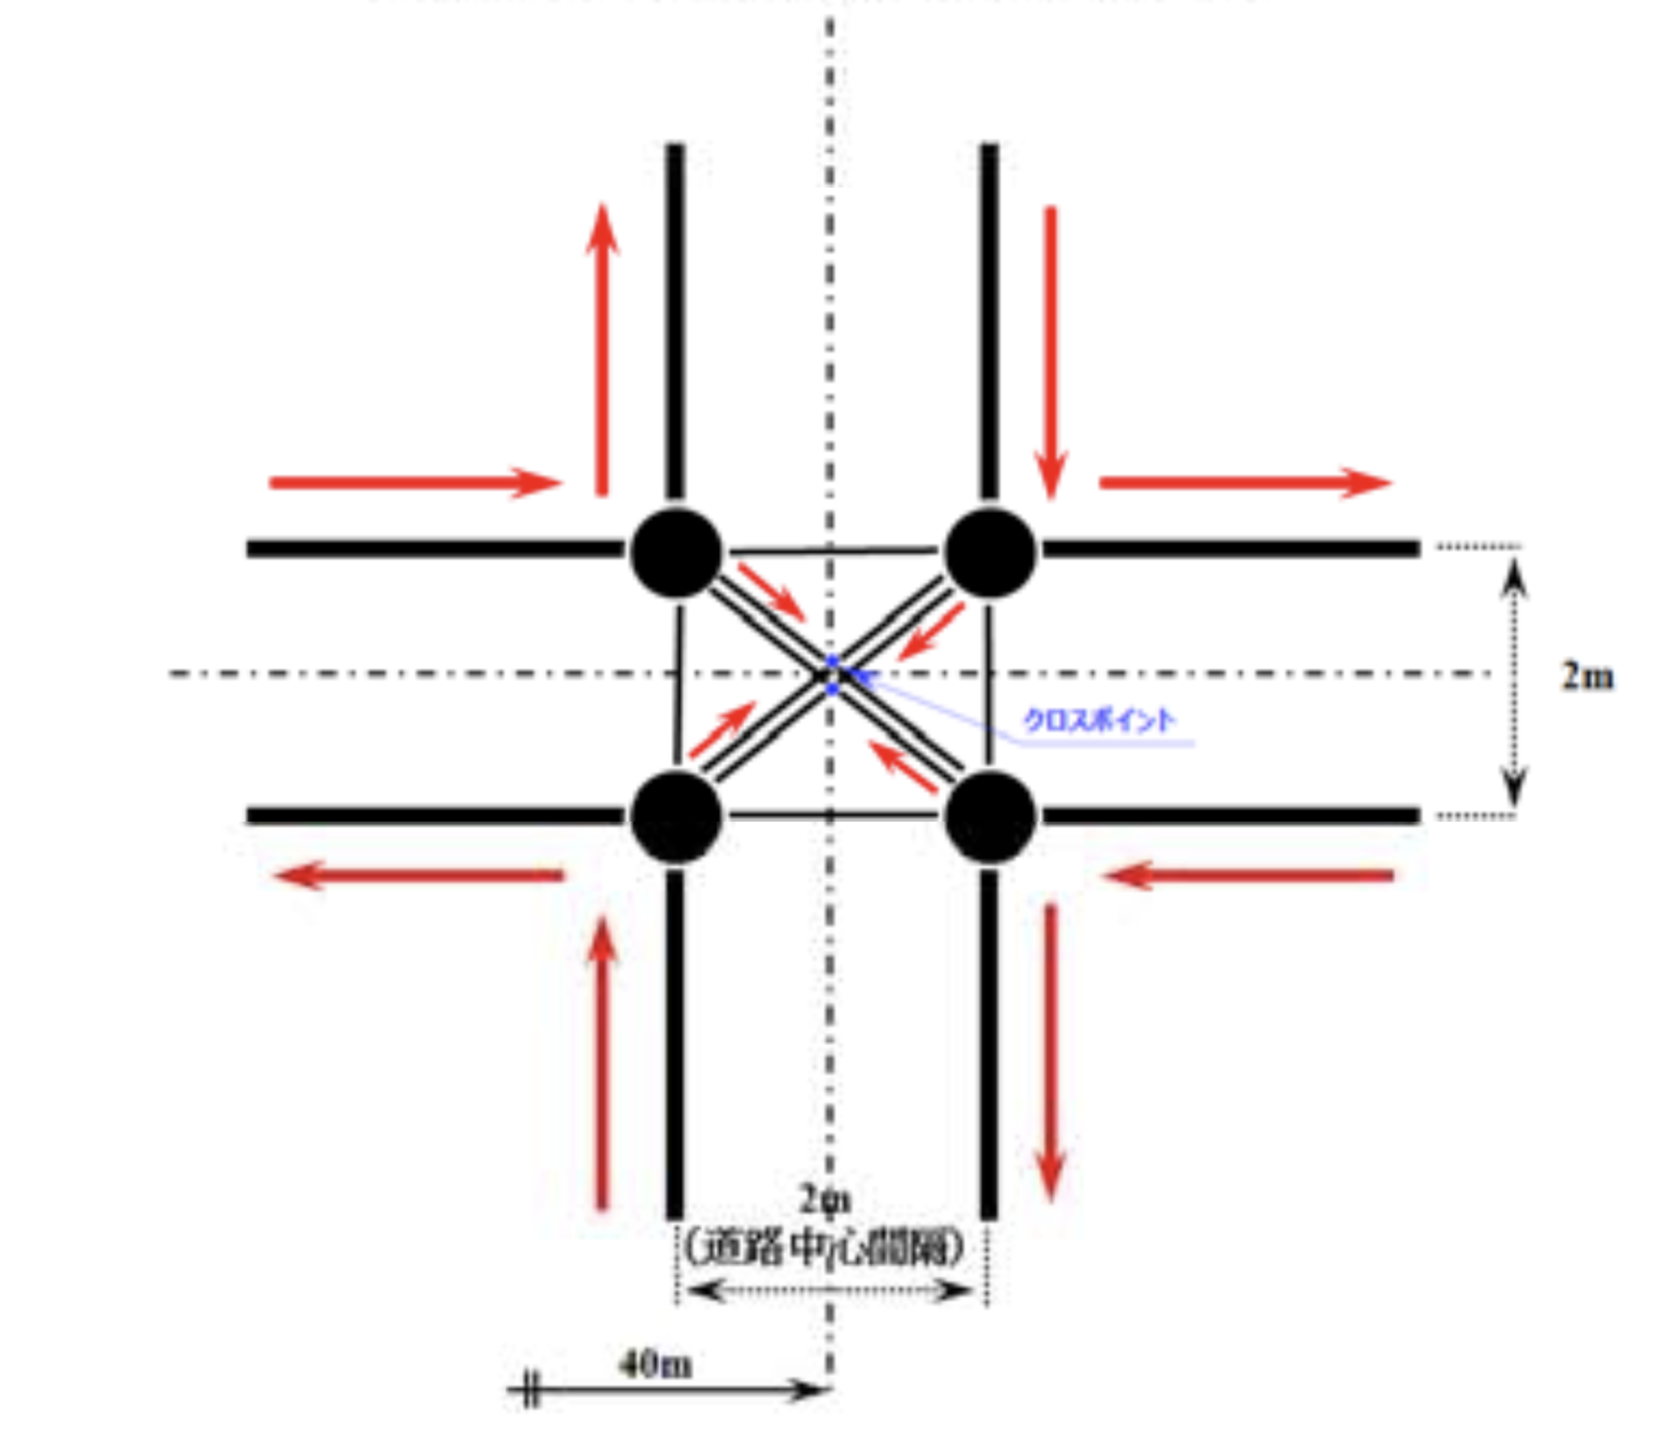
\includegraphics[width=80mm]{intermoderu.png}
	\caption{交差点の仕様}
\end{figure}
\begin{figure}
	\centering
	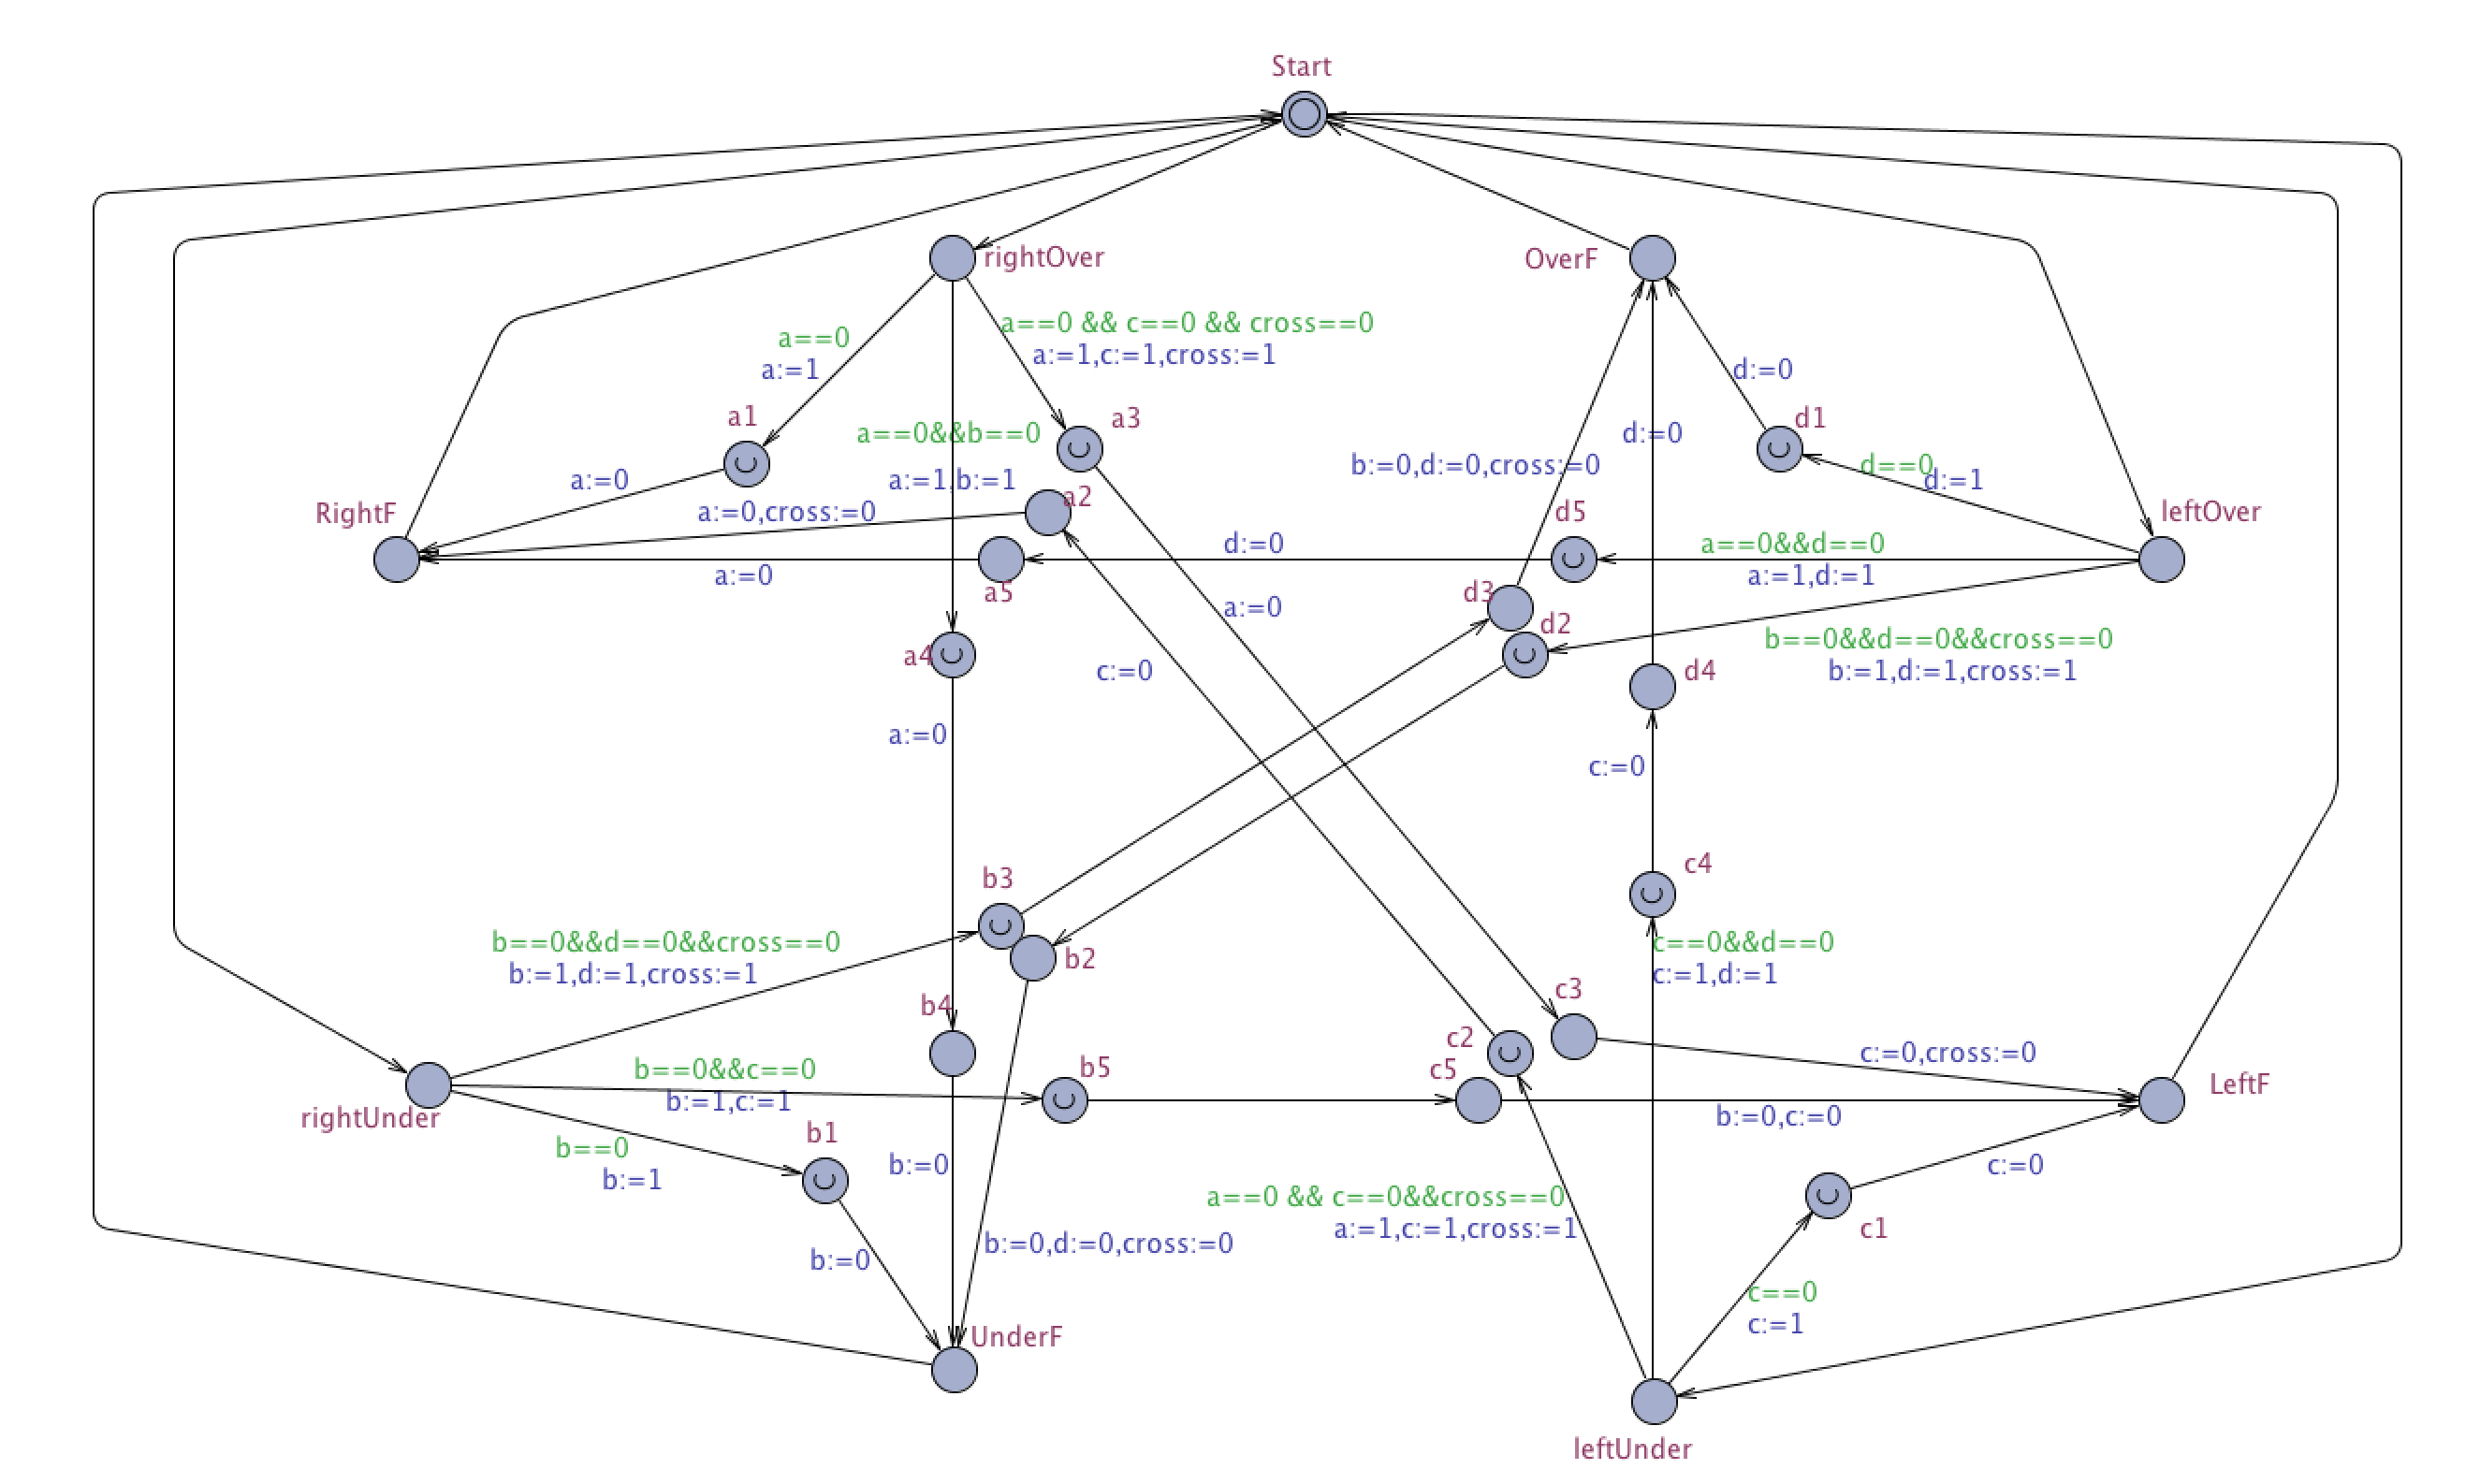
\includegraphics[width=170mm]{intersection.png}
	\caption{UPPAALによる交差点のモデル化}
\end{figure}
\begin{figure}
	\centering
	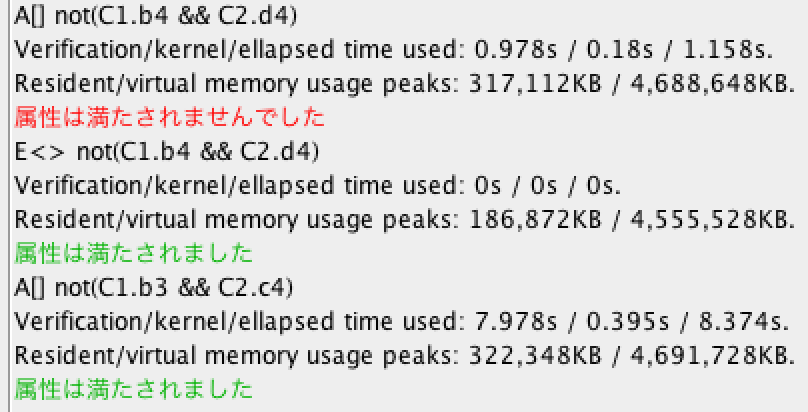
\includegraphics[width=85mm]{result.png}
	\caption{検証結果}
\end{figure}

\section*{今後の課題}
今回は時間制約条件のないモデルとしたため,次は時間制約を組み込んだものをモデル化し検証する。
\end{document}